\documentclass[preprint]{sigplanconf}
\usepackage{cleveref,amsmath,chngcntr}
\usepackage{textcomp} % for tilde
\usepackage{paralist} % for in-paragraph lists
\usepackage{url}
\usepackage{graphicx}
\usepackage{multicol,multirow}
\usepackage{tabularx}

% Make text in figure captions small
\usepackage{caption3} % load caption package kernel first
\DeclareCaptionOption{parskip}[]{} % disable "parskip" caption option
\usepackage[small]{caption}

% For drawing FSMs
%\usepackage{tikz}
%\usetikzlibrary{arrows,automata}

% Used for code snippets
\usepackage{listings,courier}
\usepackage{subfig,epsfig}
\DeclareCaptionType{copyrightbox}
\usepackage{epsfig}



% Compressed enumerations
\newenvironment{enumerate*}%
  {\begin{enumerate}%
    \setlength{\itemsep}{2pt}%
    \setlength{\parskip}{0pt}}%
  {\end{enumerate}}

% Settings on code listings.
\lstset{language=C,
		xleftmargin=0pt,
		xrightmargin=0pt,
		framexbottommargin=0pt,
        framextopmargin=0pt,
        framesep=0pt}
\usepackage{enumitem}

% Add listing language for assembly
\lstdefinelanguage
   [x64]{Assembler}     % add a "x64" dialect of Assembler
   [x86masm]{Assembler} % based on the "x86masm" dialect
   % with these extra keywords:
   {morekeywords={CDQE,CQO,CMPSQ,CMPXCHG16B,JRCXZ,LODSQ,MOVSXD, %
                  POPFQ,PUSHFQ,SCASQ,STOSQ,IRETQ,RDTSCP,SWAPGS, %
                  rax,rdx,rcx,rbx,rsi,rdi,rsp,rbp, %
                  r8,r8d,r8w,r8b,r9,r9d,r9w,r9b}} % etc.


% For leaving some comments in the draft.
\newcommand{\comment}[1]{}

% For writing Granary tool names.
\newcommand{\toolname}[1]{{\scshape #1}}

% Customize cleverref
\crefname{section}{Section}{Sections}


\begin{document}

%make title bold and 14 pt font (Latex default is non-bold, 16 pt)
\title{Fast and Flexible Binary Instrumentation for the Kernel}

%for single author (just remove % characters)
\authorinfo{Peter Goodman \and Angela Demke Brown \and Ashvin Goel}
{University of Toronto}{}
% end authorinfo

\maketitle
\subsection*{Abstract}
TODO

\section{Introduction}\label{sec:intro}

Granary is a framework for creating flexible and efficient tools that instrument the Linux kernel. Granary's key novelty is its \emph{runtime code specialization} feature, which enables tools to decide what code to instrument, and how to instrument that code. Flexible specialization allows tools to be picky about instrumentation. For example, a tool can choose to instrument every load and store operation, but only inside nested critical sections that are executing in module code. Granary's runtime code specialization feature addresses two limitations of existing kernel analysis systems: \begin{inparaenum}[i)]
	\item they have focused on instrumenting all code \cite{DRK,btkernel,QEMU}; and
	\item they can only instrument code using a single policy.
\end{inparaenum}

Instrumenting all code (e.g., the whole kernel) imposes unnecessary performance overheads when only a subset of the code is being analyzed (e.g., modules, functions). In practice, we would like to target instrumentation at specific code for efficiency, while also allowing rich and detailed instrumentation of the targeted code. Limiting the scope of what is instrumented is  important because the overhead introduced by using runtime code instrumentation is usually dominated by the instrumentation itself and not the baseline overhead of the runtime system supporting that instrumentation. Also, specializing based on what is instrumented allows instrumentation tools to focus instrumentation on the code of interest. For example, if one wants to instrument RCU read-side critical sections, as is the case with Granary's \toolname{RCUdbg} tool, then instrumenting all code just to filter out and find those critical sections is wasteful.

Another limitation of existing systems is that they are unable to perform efficient runtime code specialization. That is, they are unable to change how code is instrumented based on the context in which that code will run. This is unfortunate because it means that tools wanting to instrument code differently must create their own solution that works around this deficiency. For example, one way that existing tools can specialize code is to generate as many versions of the code as there are potential specializations. When instrumented code is executing, runtime checks continually check and jump to the correct version of the code for the current execution context. However, runtime checks are inefficient, and generating many versions of the code introduces bloat and pollutes the CPU's instruction cache. Granary avoids these issues by supporting context-specific runtime code specialization that generates multiple versions of basic blocks \emph{just-in-time} (JIT), instead ahead-of-time, and without requiring runtime checks.

One example tool that uses Granary's JIT-based runtime code specialization feature is \toolname{RCUdbg}: Granary's Read-Copy-Update (RCU) debugging tool. \toolname{RCUdbg} catches bugs related to invalid uses of RCU-protected pointers (\Cref{sec:rcudbg}). \toolname{RCUdbg} distinguishes between two kinds of RCU-protected pointers (reader-side and writer-side) and plain old pointers, and three execution contexts (inside of a read-side critical section, inside of a write-side critical section, and in non-RCU-related code). The actions taken when a pointer is de-referenced varies depending on the kind of pointer and the execution context. Code executing in read-side critical sections is specialized to enforce that only plain-old and read-side pointers are accessed, and that all accesses through read-side pointers are memory reads. Write-side critical sections are specialized in a similar way.

The \toolname{RCUdbg} tool is an example of \emph{context-driven code specialization}: code executing inside of a read-side critical section is instrumented differently from code executing inside of a write-side critical section, and code executing outside of both contexts runs natively or with lightweight instrumentation. Achieving this level of specialization using and existing system requires complicated runtime state management and checks to switch between different versions of the code. With Granary, a tool like \toolname{RCUdbg} can specialize code using \emph{instrumentation policies}. An instrumentation policy is a function that names an execution context and decides how to instrument instructions that will execute within that context. When a policy is used to instrument a sequence of instructions (called a basic block), a new version of the basic block is generated and cached. 

\toolname{RCUdbg} defines three policies, and declares transitions between these policies when control flows in and out of RCU read- and write-side critical sections. When a function like \texttt{memset} is invoked in one context, the policy associated with that context is used to generate an instrumented version of \texttt{memset} for that context. If, for example, \texttt{memset} is never invoked within a read-side critical section, then \texttt{memset}'s code will never be specialized to perform the heavyweight checks needed to detect RCU-protected pointer misuses in this context. Similarly, if \texttt{memset} is executed both in a write-side critical section and outside of any RCU-related code, then two differently instrumented versions of \texttt{memset} will be generated.

The key insight of Granary's approach to runtime code specialization is that code versioning is a context-tracking mechanism. That is, if an instruction from a basic block instrumented by \toolname{RCUdbg}'s read-side critical section policy is being executed, then the current thread must be executing inside of a read-side critical section. Similarly, if the read-side policy is used to instrument a basic block, then \texttt{RCUdbg} knows at instrumentation time\footnote{Instrumentation time is analogous to ``compile time", in that a policy is generally used to instrument a basic block of code once, and then that basic block may be executed many times.} that this basic block will only execute within a read-side critical section. If the basic block contains a \texttt{call} to the \texttt{memset} function, then \texttt{memset} is also known to execute within a read-side critical section because it does not terminate a read-side critical section. By deciding which version of \texttt{memset} to execute at instrumentation time, \toolname{RCUdbg} avoids expensive runtime checks that other systems impose in order to achieve similar kinds of specialization. \toolname{RCUdbg} can specify that \texttt{memset} will also execute within a read-side critical section by telling Granary that it should use the read-side critical section policy to instrument \texttt{memset}. 

The rest of the paper describes Granary in more detail. \Cref{sec:dbt} describes how Granary is implemented, \Cref{sec:what} describes how a Granary tool can choose to instrument only specific code, \Cref{sec:how} describes how Granary change the policy used to instrument code, etc.

\section{Dynamic Binary Translation}\label{sec:dbt}

Granary uses dynamic binary translation (DBT) to instrument the Linux kernel. DBT is used for emulation \cite{QEMU}, runtime optimization \cite{DynamoRIOOptimization}, and runtime instrumentation (analysis \cite{DynamoRIO, DRK, btkernel, ProfilingSimics}, security \cite{Vx32,NaCl,ProgramShepherding}, and debugging \cite{Valgrind}). We chose DBT because \begin{inparaenum}[i)]
	\item static binary analysis tools are unable to cope with \texttt{x86-64}'s mix of variably-sized instructions and data; 
	\item some kernel code is only distributed in a binary format (e.g. proprietary device drivers); and
	\item virtualization-based approaches are unable to analyze non-virtualizable device drivers \cite{DRK}.
\end{inparaenum}

Granary translates and instruments kernel binaries one basic block at a time. In Granary, a basic block is a sequence of x86-64 instructions ending in a conditional branch (\texttt{jCC}), \texttt{ret}, or a \texttt{jmp} instruction. Unlike DRK and btkernel, Granary does not terminate basic blocks at \texttt{call} instructions. This enables longer basic blocks and native-like proceccor return address prediction, but makes Granary non-transparent (\Cref{sec:transparency}). Granary takes control of execution starting from ``natural" program entrypoints (e.g. interrupt vectors, system call entrypoints, module initializers). Entrypoint basic blocks  are translated ahead-of-time, and all other basic blocks are translated just-in-time (JIT) as control flow reaches them for the first time.

Translated basic blocks are linked together and stored in a \emph{code cache}. Basic blocks are indexed by $(pc, policy)$ pairs, where $pc$ is the native program counter associated with the beginning of the basic block's instructions, and $policy$ is the instrumentation policy used to instrument the native instructions starting at $pc$. The index is maintained by a globally accessible hash table.

Granary's JIT-based translation approach means that code executing from the code cache may yield control to Granary to request the address of the next basic block to execute. This happens when there is a control flow transfer in a basic block, and the target of that control flow transfer is not already indexed in Granary's code cache. When instrumented code yields to Granary, a ``context switch'' occurs that transfers execution to a CPU-private stack where Granary operates. Granary operates on a CPU-private stack for two reasons. First, if Granary did not switch stacks, then context switches into Granary risk overflowing the runtime call stack. This can happen because kernel stacks are typically small (4K to 8K in size), and because a context switch could happen when the native stack is nearly exhausted. Second, on an SMP, multiple processors can simultaneously execute Granary code (e.g. to translate code that will later execute). In such cases, Granary depends on CPU-private data structures to avoid contention, and the private stack is one such data structure. A context-switch back to the code cache occurs when the next basic block has been found or translated. At this point, instrumented execution continues. Similar to other DBT systems, Granary uses hot code patching (also called code splicing) to reduce the number of context switches. In our experience, kernel code stabilizes very quickly: context switches stop happening after the first few seconds of translation.

\subsection{Basic Block Meta-Data}\label{sec:metadata}

Associated with each basic block is meta-data that describes the basic block. Basic block meta-data includes: \begin{itemize}
	\item The length in bytes of the original and translated basic blocks, and the address of the first instruction in the original basic block and the instrumented basic block. This information helps provide a rich debugging interface for instrumentation tool authors. Granary is unique among DBT tools in that the debugging experience is actually pleasant. For example, Granary has a built-in reverse debugging mechanism, which allows developers to inspect previously executed basic blocks and past register state.
	\item Linux kernel-specific exception table meta-data about instructions contained within the current basic block. This kernel-specific meta-data is used by Granary to implement transparent page fault exception handling (\Cref{sec:interrupt_return_address_transparency}).
	\item Ranges of instructions that must be executed atomically. Granary uses this information to implement selective interrupt delaying (\Cref{sec:interrupt_delay}).
	\item The allocator used to allocate the instructions of the basic block. Granary uses this information to implement its trace-allocation optimization (\Cref{sec:trace_alloc}).
	\item The instrumentation policy used to instrument the basic block. Granary uses this information to allow instrumentation tools to define policy-specific interrupt handling routines. For example, \toolname{RCUdbg} implements a read-side policy-specific interrupt handling routine that reports an error if code executing within a read-side critical section is interrupted (\Cref{sec:rcudbg}).
\end{itemize}

Basic block meta-data can also be extended by instrumentation tools. This makes developing instrumentation tools that record per-basic block statistics very easy to make. For example, Granary's control-flow graph tool, \toolname{cfg}, extends the basic block meta-data to track per-block and per-edge execution counts (\Cref{sec:cfg}). This data is useful because it provides precise code coverage information (block and branch coverage), as well as useful data for profile-guided optimization. This meta-data is specified by \toolname{cfg} and automatically allocated by Granary. 

\subsection{Transparency}\label{sec:transparency}
An instrumentation system is transparent if, given the same inputs, the instrumented and uninstrumented versions of a program behave in the same way \cite{Transparency}. Granary includes configurable levels of transparency to address the trade-off between transparency and overhead. By default, Granary uses a relaxed transparency \cite{btkernel} model for efficiency, flexibility and increased visibility, but if instrumentation for some module requires transparency then it can be enabled at the cost of increased overheads and decreased visibility. By default, the only artifact Granary exposes is that interrupt and function return addresses can point into the code cache.

\subsubsection{Function return addresses}\label{sec:return_address_transparency}
Unlike most DBT frameworks, Granary's basic blocks do not terminate at \texttt{call} instructions. This exposes code cache addresses to instrumented module code in the form of return addresses stored on the runtime call stack. The benefit of including \texttt{call} instructions are: \begin{enumerate}

	\item {\bf Zero overhead procedure returns.} Unlike Granary, DRK emulates procedure calls and returns. DRK emulates \texttt{call} instructions by pushing the intended native return address onto the runtime call stack, followed by a direct direct jump to the next (instrumented) basic block \cite{DRK}. This approach enables return address transparency, but introduces additional overheads on procedure returns, which must do costly indirect branch lookups to find the intended return target. 

Btkernel's approach is similar in spirit to Granary's; however, btkernel ends basic blocks at \texttt{call} instructions. This introduces unnecessary control-flow on the return path from procedures. That is, btkernel's ``call/ret optimization" ostensibly enables zero-overhead procedure returns by leaving \texttt{ret} instructions as-is; however, the benefits are more apparent than real. To transfer control to the next logical basic block after a procedure return, btkernel's \texttt{ret}s first transfer control to the end of the basic block that performed the \texttt{call}, and then \texttt{jmp} to the next basic block. Granary avoids this unnecessary \texttt{jmp} because basic blocks do not end at \texttt{call} instructions.
	
In some cases, emulating DRK's return-address lookup mechanism is desirable. For example, if Granary attaches while some program's execution is underway (and so the runtime call stack contains native return addresses), then a direct \texttt{ret} back to one of the native return addresses might be undesirable (e.g. if the tool wants comprehensive instrumentation of all code). In such cases, a tool can partially specialize instrumentation according to whether or not the return address might be in the code cache. Partial specialization is enabled by \emph{policy properties}, which are transparently inherited along with normal instrumentation policy information. In this case, the policy property can be used to tell Granary to emulate \texttt{ret} instructions when the return address is potentially a native address, and directly \texttt{ret} when the return address is known to be in the code cache.\footnote{This feature is used when Granary is configured to instrument user space programs. User space Granary depends on the Linux dynamic loader to inject Granary into a running process. When injected, a Granary takeover function is executed on an already active native runtime call stack. Granary's takeover procedure transparently emulates returns, thus taking over the previously fully-native call stack. This feature allows instrumentation tools to focus on their particular objectives and not the intricacies of thread takeover.}

	\item {\bf Improved visibility.} Not ending basic blocks on \texttt{call} instructions results in longer basic blocks, which in turn provide additional visibility to tools at instrumentation time into what will be executed by the current thread. \toolname{RCUdbg} benefits from this additional visibility because it can observe the end of read-side critical sections (\texttt{call}s to \texttt{rcu\_read\_unlock}), and optimistically assume that functions executing before the read-side critical section ends will execute within the read-side critical section.

\end{enumerate}

\subsubsection{Interrupt return addresses}\label{sec:interrupt_return_address_transparency}
Kernel interrupts are not sensitive to return addresses and hence relaxing return address transparency has no effect on interrupts. A special case arises for page fault exceptions that occur within specific kernel functions that access user space data \cite{btkernel}. The Linux kernel records ranges of code addresses that are permitted to fault in an ``exception table'' data structure, and on a page fault exception, checks if the exception return address belongs to one of the pre-defined ranges. Granary records any exception table entries as part of each basic block's meta-data, so that a page fault in a basic block can be mapped to the correct native faulting program counter.

\subsection{Reentrancy}
Reentrancy is an important concern for all DBT systems, and is especially important for DBT systems operating in the kernel environment. For example, hardware interrupts can redirect control flow at any instruction, and interrupt delivery cannot be delayed past the execution of memory instructions that might alter the interrupt delivery state \cite{DRK}. Preserving interrupt transparency, however, requires that interrupts either be delayed until the end of any injected instrumentation instructions. Together, these requirements make it very difficult to write instrumentation tools.

\subsubsection{Granary}
For efficiency, most kernel-space instrumentation systems (Granary included) operate on CPU-private state (e.g. Granary's CPU-private stacks). However, accessing CPU-private data without first disabling interrupts results in undefined behavior. Therefore, context-switches into Granary first disable interrupts and then switch execution onto one of Granary's CPU-private stacks. Context switches out of Granary and into native code or the code cache returns execution to the native stack and re-enable interrupts. Execution behavior is preserved because Granary saves the machine state (i.e. registers, flags) in a reentrant way. All other parts of Granary are fully reentrant.

\subsubsection{Instrumentation}\label{sec:interrupt_delay}

\begin{figure}[t!]
\begin{multicols}{2}
\vspace{-1.5em}\subfloat[\label{fig:interrupt_delay_drk}Pre and post instrumentation in DRK. Injected instrumentation blocks are treated as atomic with respect to interrupts.]{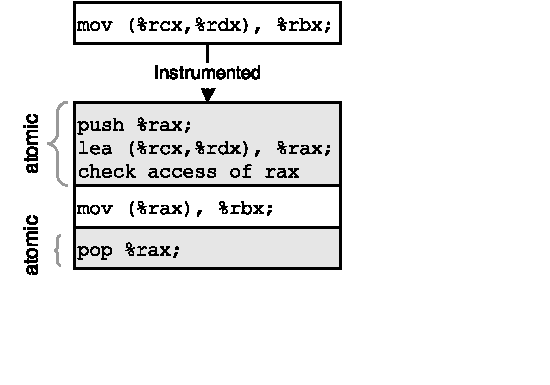
\includegraphics[height=10em,clip=true,trim=0 5em 10em 0]{diagrams/drk_instrumented_mov.pdf}}\vspace{-2.5em}
\columnbreak
\vspace{-1.5em}\hspace{-0.5em}\subfloat[\label{fig:interrupt_delay_granary}Pre and post instrumentation in Granary. The two instrumentation blocks, as well as the native instruction are wrapped in a delay region.]{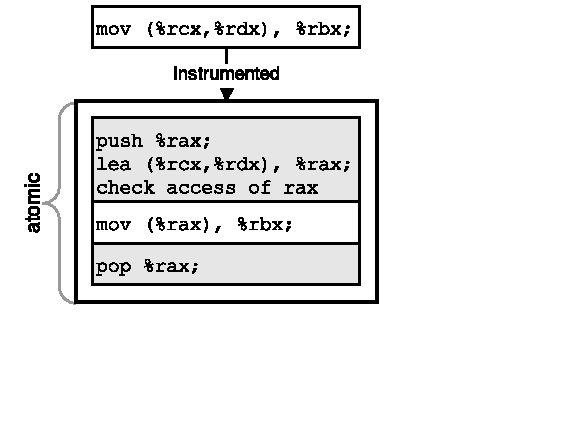
\includegraphics[height=10em,clip=true,trim=0 5em 10em 0]{diagrams/granary_instrumented_mov.pdf}}\vspace{-2.5em}
\end{multicols}
\caption{Example showing equivalent pre- and post-instruction instrumentation with DRK (left) and Granary (right). In DRK, the injected instrumentation instructions (grey) are guaranteed to execute atomically, up until the next native instruction (white). In Granary, no guarantees are made on injected instrumentation, unless otherwise instructed. In this case, a delay region surrounds both the pre- and post-instrumentation, as well as the native instruction, guaranteeing that the entire sequence of instructions execute on the same CPU.}
\end{figure}

One challenge with any DBT system is how it copes with non-reentrant instrumentation. For example, instrumentation that modifies CPU-private data structures (without disabling interrupts) cannot be safely executed by a pre-emptive kernel running on an SMP. If the thread being instrumented is interrupted, then the kernel might decide to re-schedule the thread to resume its execution on a different CPU. Any modifications to CPU-private state would lead to undefined behavior. An example of this is instrumentation that acquires a CPU-private lock on one CPU, is interrupted, and later releases the wrong lock on the wrong CPU.

DRK's solution to this problem assumes that all injected instrumentation instructions are potentially non-reentrant, and \emph{delays} interrupts occuring within instrumented code \cite{DRK}. Interrupt delaying allows DRK to maintain the precise interrupt semantics of x86-64: interrupts and exceptions only arrive on native instruction boundaries, and kernel interrupt handlers only observe faults or exceptions at native instruction boundaries. This approach introduces subtle complexity when injecting non-idempotent instrumentation before (pre) and after (post) native instructions.

\Cref{fig:interrupt_delay_drk} shows an example of pre- and post-instrumentation around a \texttt{mov} instruction. If an interrupt arrives within the pre-instrumentation, then DRK delays they delivery of the interrupt until the native instruction (\texttt{mov}). After the interrupt is handled and execution attempts to return to the interrupted instructions, DRK will re-instrument the ``tail" of interrupted basic block, starting from the \texttt{mov} instruction. This involves re-creating the pre- and post-instrumentation of the \texttt{mov} in the tail basic block. When executed, this will result in an unbalanced number of \texttt{push} and \texttt{pop} instructions. That is, \texttt{push \%rax} is executed in both the original and tail basic block, but \texttt{pop \%rax} is only executed in the tail basic block. This is a specific example of a more general problem: DRK's approach to interrupt delaying does not play well with non-idempotent instrumentation.

Btkernel provides no solution to the problem of handling non-reentrant instrumentation, beyond requiring that instrumentation tools disable and re-enable interrupts around non-reentrant instrumentation code \cite{btkernel}. The is inefficient because it introduces flag stalls into the instruction pipeline \cite{AgnerMicroarchitecture}, and because interrupts arrive relatively infrequently.

Granary charts a middle ground between the two aforementioned approaches. Most instrumentation is re-entrant, partially because kernel instrumentation tools can depend on the runtime call stack for scratch storage space. However, interrupt delaying is sometimes useful because it enables non-reentrant instrumentation to avoid having to continually disable and re-enable interrupts. For example, Granary's \toolname{Guardrail} tool records traces of executed module instructions into CPU-private buffers \cite{Guardrail}. These traces are concurrently analyzed for bugs by another thread. Operating on a CPU-private buffer is more efficient than operating on a global buffer because it avoids cache line contention and locking on an SMP. However, writing to a CPU-private buffer is only safe if the entire write executes on the same CPU. An equivalent tool developed for btkernel---which does not support interrupt delaying---would have to disable and the re-enable interrupts around the write. 

Granary conveniently solves this problem by allowing instrumentation tools to declare \emph{interrupt delay regions}. An interrupt delay region is a sequence of instructions (which can contain internal control flow) inside of a basic block that must be executed atomically. \Cref{fig:interrupt_delay_granary} shows an interrut delay region that surrounds both the pre- and post-instrumentation of a native \texttt{mov} instruction. If an interrupt arrives anywhere within this region of code, Granary will delay the interrupt to the end of the region. The declarative nature of interrupt delay regions allows instrumentation developers to opt-in to interrupt delaying, and control exactly when, where, and for how long interrupts can be delayed.

Granary implements interrupt delay regions by recording bounds information about interrupt delay regions inside of each basic block's meta-data (\Cref{sec:metadata}). When a basic block is interrupted, Granary inspects the block's meta-data and determines if the interrupt must be delayed. If a delay is required, then all instructions belonging to the delay range are copied into a CPU-private buffer. All instructions are copied because a delay region might contain internal control-flow. A CPU-private buffer is used because the number of CPUs is a natural upper bound on the number of simultaneously executing delay regions. After the copied instructions, Granary emits code that code re-creates the interrupt stack frame, followed by a jump to the interrupt vector (which is controlled by Granary). This jump ensures that Granary's interrupt handler regains control after the instructions within the delay region fully execute, but before the kernel observes the interrupt. When Granary regains control, it can then delegate to the instrumentation tool to handle the interrupt, or defer handling of the interrupt to the kernel.

When all instructions have been emitted to the CPU-private buffer, Granary emulates a return from the interrupt (without issuing an \texttt{iret} instruction). The emulated return leaves interrupts disabled and transfers control to the CPU-private buffer. Leaving interrupts disabled ensures that the remainder of the delay region will execute on the current CPU, and avoids reentrancy issues related to the copied region being located in a CPU-private buffer.

\subsection{Control Flow Implementation}

Granary's mechanism of looking up branch targets and resolving control flow depends only on control flow instruction (CTI) policy and target information. This information is either directly embedded in emitted executable code, or in immutable data structures directly referenced by emitted code. This approach ensures that policy information is never lost or corrupted, even in the face of concurrent executions of the same emitted code, arbitrary pre-emption, and arbitrary resumption. Because Granary's translation mechanism is driven by these two inputs, Granary is otherwise stateless\footnote{This is not quite true, as Granary maintains persistent state in the form of the code cache index. However, the code cache index behaves similarly to memoization in a purely functional programming language: it is an optimization, not a necessity.} across context switches.

\subsubsection{Direct Control Flow}\label{sec:direct_control_flow}
\lstset{language=[x64]Assembler}
\newsavebox\nativejcc
\begin{lrbox}{\nativejcc}
\begin{minipage}[b]{4cm}
\begin{lstlisting}[basicstyle=\scriptsize\ttfamily]
cmp $0x0, %rax
jz value_is_zero 
...
( fall through )
\end{lstlisting}
\end{minipage}
\end{lrbox}

\newsavebox\translatedjcc
\begin{lrbox}{\translatedjcc}\begin{minipage}[b]{4cm}\begin{lstlisting}[basicstyle=\scriptsize\ttfamily]
  cmp $0x0, %rax
  jz edge_value_is_zero
  jmp edge_fall_through

edge_value_is_zero:
  call *(jz_patch_data)
edge_fall_through:
  call *(jmp_patch_data)
\end{lstlisting}
\end{minipage}
\end{lrbox}

\begin{figure}[t!]
\subfloat[Native Code]{\usebox\nativejcc}
\hfill
\subfloat[Translated Code]{\usebox\translatedjcc}
\caption{\label{fig:direct_edge_code}Example translation of a conditional control flow instruction (\texttt{jz}) and its edge code. The original \texttt{jz} is translated into a \texttt{jz} that uses a 32-bit relative displacement to transfer control to an edge code function call (\texttt{edge\_value\_is\_zero}). When executed, the function call reads its target from an edge data structure (\texttt{jz\_patch\_data}), which contains all information necessary to resolve the \texttt{jz}'s target and patch the original \texttt{jz}. Patching is performed with a four byte atomic write to the relative displacement operand of the \texttt{jz} instruction. Finally, the return address of the \texttt{call} instruction is altered to transfer control to the newly resolved target.}
\end{figure}
Like btkernel, Granary translates direct CTIs into equivalent jumps into CTI-specific ``edge code" (\Cref{fig:direct_edge_code}). Edge code lives outside the code cache, so as to not pollute the processor's instruction cache \cite{btkernel}.

When control flows through a basic block $B_{pred}$ for the first time, any jumps taken will transfer control to edge code that is specific to the jump taken. Edge code contains only a single indirect \texttt{call} instruction, thus allowing multiple edge codes to occupy a single cache line. The indirect \texttt{call} transfers control to Granary via a function pointer located in an ``edge data structure", which describes how to translate the target basic block, $B_{succ}$. Granary gains control and looks up or translates the target code according instrumentation policy stored in the edge data structure. Then, Granary modifies the original CTI in $B_{pred}$ so that it transfers control to $B_{succ}$  (\Cref{sec:patching}). Finally, Granary releases control and context switches to $B_{succ}$.

\subsubsection{Indirect Control Flow}\label{sec:ibl}

Granary translates indirect CTIs (\texttt{call}, \texttt{jmp}) into their equivalent direct control flow versions, where the direct versions branch to ``in-edge" code. In-edge code loads the indirect jump target (e.g. a specific register or memory location), saves the flags register, and several scratch registers. Finally, the in-edge uses the indirect target as an index into a global, fixed-size hash table of indirect branch targets. The entries of the hash table either point to Granary or to ``out-edge" code (\Cref{fig:ibl}). 

\begin{figure}[t!]
\hspace{4em}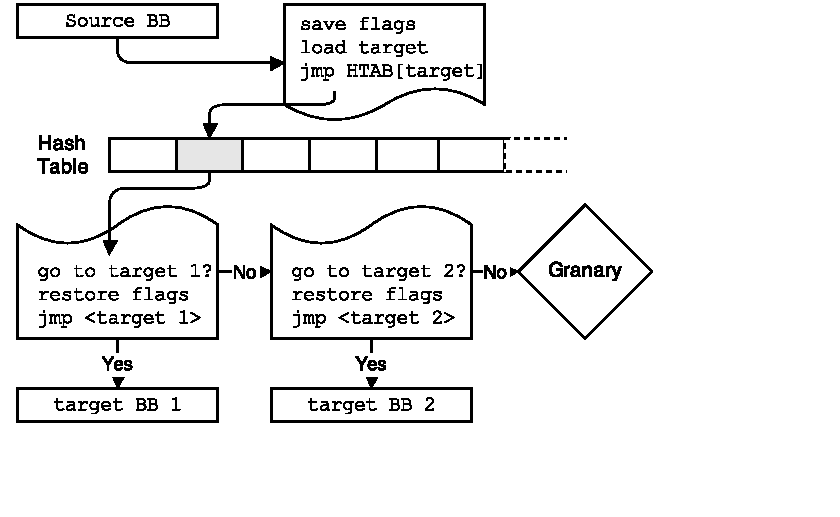
\includegraphics[height=13em,clip=true,trim=0 5em 10em 0]{diagrams/ibl.pdf}
\caption{\label{fig:ibl}Process of resolving an indirect branch. Control transfers from a source basic block, to the in-edge code specific to where the indirect target is stored (e.g. register, memory address), through the global hash table and on to either one or more out-edge code stubs, or to Granary.}
\end{figure}

Out-edge code is specific to a target basic block, and performs the function of separate chaining in the indirect branch lookup hash table. When control transfers to out-edge code, the out-edge checks to see if the indirect target matches the out-edge code's target basic block. If they match, then the out-edge code restores scratch and flags registers and jumps directly to the target basic block. Otherwise, the out-edge code jumps to another out-edge code or to Granary. If one out-edge code block jumps to another one, then the targets of the two out-edge code blocks collide in the global hash table. In this respect, out-edge code is chained together through control flow, just as colliding entries in a typical hash table can be chained together through a linked list.

Granary's use of out-edge code avoids re-entrancy issues related to indirect control flow that are present in DRK and btkernel. Both DRK and btkernel store the target of an indirect CTI in a CPU-private memory location. To complete an indirect control transfer, both systems perform (roughly) the following steps: \begin{enumerate}[itemindent=\parindent]%
\setlength{\itemsep}{2pt}%
\setlength{\parskip}{0pt}%
	\item Save the flags and disable interrupts.
	\item Save registers.
	\item Lookup the next basic block address.
	\item Store that address in a CPU private memory location.
	\item Restore registers.
	\item Restore the flags and interrupt state.
	\item Indirectly jump to the target basic block through the CPU-private location.
\end{enumerate} %
However, the ordering of steps (6) and (7) introduce a reentrancy problem: the access to the CPU-private location is not safe because an interrupt might arrive before the indirect jump in step (7). This unusual design is motivated by the constraint that the entire lookup procedure must save (2) and restore (5) the register state for correctness, but must also save the target pc \emph{somewhere} so that execution can eventually be redirected. Granary's out-edge code avoids this reentrancy issue by having the out edge code itself (in the form of a direct \texttt{jmp}) contain the target pc.

\subsection{Optimizations}

\subsubsection{Ahead-of-time Translation Optimization} \label{sec:aot}
Granary ends basic blocks at conditional branches (\texttt{jCC}), direct and indirect \texttt{jmp}s, and \texttt{ret}s and \texttt{iret}s. Basic blocks ending in conditional branches are extended to contain two trailing CTIs: a copy of the native \texttt{jCC}, and a synthesized direct \texttt{jmp} to the code executed when the condition code is not set (i.e. when the conditional jump is not taken).

If a basic block ends in either a copy of a native direct \texttt{jmp} or synthesized direct \texttt{jmp}, then Granary will perform ahead-of-time translation and instrumentation of the targeted basic block. The repeated application of translating \texttt{jmp} targets forms traces in Granary's code cache. Granary optimizes traces by directly connecting basic blocks together when there is internal control flow within the blocks of the trace, and by eliding \texttt{jmp}s between adjacent basic blocks.

Granary's tracing strategy is based on the observation that the most commonly executed path through code follows a straight line. That is, execution is more likely to fall through a conditional CTI than it is to take the conditional CTI. We experimentally verified Granary's tracing strategy by disabling tracing and relying on Granary's internal performance counters to count how many conditional branches were patched (by their edge code, \texttildelow 25\%), versus how many synthesized fall-through \texttt{jmp}s were patched (\texttildelow 80\%).

\subsubsection{Patching and Alignment  Optimizations}\label{sec:patching}
For efficiency, basic blocks in Granary's code cache are directly connected through direct control flow instructions (\texttt{call}, \texttt{jmp}, \texttt{jCC}). That is, if there is a direct branch from one native instruction to another, then there will be a corresponding direct branch in the translated code.

Granary opportunistically connects two basic blocks together using a direct branch when: \begin{inparaenum}[i)]
	\item the branch transfers control to another basic block within the current trace; or
	\item the branch transfers control to an already translated basic block.
\end{inparaenum} However, not all basic blocks can be connected at translation time, therefore Granary employs edge code and hot-code patching (\Cref{fig:direct_edge_code}) to connect basic blocks at runtime.

Granary atomically patches direct CTIs that target edge code to instead point to their (now resolved) target basic block. Due to limitations of the x86-64 architecture, atomic operations cannot straddle cache lines. Therefore, patchable instructions (or parts thereof) must be aligned so as to not straddle two cache lines.

One approach to change an instruction's alignment is to pad the basic block with additional \texttt{nop} instructions. An alternative when more than a few bytes of padding are needed is to introduce a single control-flow instruction (\texttt{jmp}) that jumps around the padded area. However, adding extra instructions introduces latency into the processor's fetch/decode/execute cycle. Therefore, when possible, Granary uses ignored instruction prefixes to alter an instruction's alignment. For example, Granary aligns patchable conditional jumps using static branch prediction hint prefixes, which are ignored by recent x86-64 processors \cite{AgnerMicroarchitecture}. Finally, most basic blocks are small (i.e. fit in one cache line), therefore, aligning basic blocks on cache line boundaries naturally avoids the potential for a patchable instruction to straddle two cache lines.

\subsubsection{Trace Allocation Optimization}\label{sec:trace_alloc}
Arranging for commonly executed sequences of basic blocks to appear adjacent in memory, also called tracing, typically improves the runtime performance of instrumented programs \cite{DynamoRIO}. Typical approaches to tracing require a runtime profiling infrastructure \cite{DynamoRIOOptimization}. Granary attempts to reap the benefits of tracing without the runtime profiling overhead by opportunistically forming traces using ahead-of-time translation (\Cref{sec:aot}), and by arranging for related basic blocks to be allocated sequentially in memory.

Two basic blocks $B_1$ and $B_2$ are ``related" ($B_1 \to B_2$) if there is a control flow instruction from $B_1$ to $B_2$. Granary arranges for $B_2$ to be allocated nearby or adjacent to $B_1$ by allocating $B_2$'s instructions from the same pool of memory used to allocate $B_1$'s instructions. The base case of this induction are kernel entrypoints. For example, each system call is an entrypoint into the kernel, and is associated with a private memory pool. When a system call is executed for the first time, the basic blocks needed to fulfill the system call's computation are allocated from that system call's memory pool.

To avoid translation conflicts (e.g. on utility functions being simultaneously executed by distinct system calls), and to improve the predictability and reproducability of a given code cache layout, Granary can delay the takeover of kernel entrypoints. That is, Granary can take over one entrypoint at a time, and wait for a specified period of time before taking over the next entrypoint. The effect of delaying the takeover process is that it increases the chances that a given entrypoint (e.g. a blocking system call) will execute to completion, and thus have all of its basic blocks  arranged sequentially in memory.

Trace allocation is implemented by recording the memory pool used to allocate a given basic block in that basic block's meta-data (\Cref{sec:metadata}). When Granary needs to translate a new basic block, it inspects the predecessor basic block's meta-data and uses the predecessor basic block's memory pool to service allocation requests for the basic block in translation.

\subsubsection{System Call Table Optimization}

Granary treats indirect \texttt{jmp}s or \texttt{call}s through the Linux kernel system call table specially. The Linux kernel (as of Linux 3.12) has approximately 300 distinct system call targets, some of which are executed often. To avoid polluting the indirect branch lookup hash table with these targets (\Cref{sec:ibl}), and to avoid the indirect branch lookup overhead, Granary creates a separate, \emph{shadow} system call table.

Granary's translation post-processing mechanism identifies indirect control flow through the system call table and alters those CTIs to direct control flow through the shadow system call table instead. The entries of the shadow system call table are ``lazy" entrypoint translator functions. Upon their first execution, these entrypoint translators find or translate the first basic block of the system call handler, and update the shadow system call table accordingly. 


\begin{table*}[ht!]
\scriptsize
\begin{tabularx}{\linewidth}{| l | >{\raggedright}p{0.3\linewidth} | X |}
\hline
\bf Granularity & \bf Description & \bf Example Tool \\
\hline
Kernel & All kernel code is instrumented. & Granary's \toolname{cfg} tool constructs inter- and intra-procedural control flow graphs and records per-basic block and per-edge performance counters. This data is useful for debugging an performance analysis. Applying the \toolname{cfg} tool to the whole kernel allows us to perform profile-guided optimization of kernel code, including a form of de-virtualization. That is, most indirect control flow instructions (\texttt{call}, \texttt{jmp}) within the kernel target only one destination. Fast checks can be inlined into kernel code that use direct control transfer instructions when possible, and fall-back on indirect control transfer instructions when necessary.\\
\hline
Module & All code from a specific kernel module or driver is instrumented. Granary detaches when module code invokes kernel code, and re-attaches when kernel code invokes module code. All non-module kernel code executes with zero overhead. & Granary's \toolname{Guardrail} tool records traces all instructions and memory operations performed by device driver code \cite{Guardrail}. A sideline thread analyzes the recorded traces to detect data race bugs and memory access bugs. \\
\hline
Function & All code within a particular function is instrumented. Granary attaches when the function is invoked, and detaches when the function returns or invokes another function. & \toolname{RCUdbg} interposes on the \texttt{rcu\_\linebreak[0]read\_\linebreak[0]lock} and \texttt{rcu\_\linebreak[0]read\_\linebreak[0]unlock} Linux kernel functions. When invoked by native code, \texttt{rcu\_\linebreak[0]read\_\linebreak[0]lock} attaches instrumentation. When invoked by instrumented code, \texttt{rcu\_\linebreak[0]read\_\linebreak[0]lock} updates the current nesting depth of the read-side critical section. \\
\hline
\end{tabularx}
\caption{\label{tab:granularities}Different granularities of instrumentation supported by Granary.}
\end{table*}

\section{Only Instrument What is Needed}\label{sec:what}

Some instrumentation tools have a limited scope, and therefore do not need to instrument all code. For example, Granary's \toolname{Guardrail} tool is concerned with finding bugs in Linux device drivers \cite{Guardrail}. \toolname{Guardrail} records traces of executed instructions, and analyzes those traces to find memory access and concurrency bugs. Both phases are heavyweight, and so limiting the scope of what is instrumented to what is of interest (module code) results in better performance. Unfortunately, existing systems are unable to change the granularity of instrumentation. Fortunately, Granary allows \toolname{Guardrail} to set the granularity of instrumentation to only instrument a specific module, while leaving the rest of the kernel to execute without overhead.

\toolname{Guardrail} is an example of how tools can choose the instrumentation granularity that best matches their needs. That is, a Granary tool can choose to instrument some code, while leaving other code to execute natively. This is useful when the instrumentation in question has a high overhead or when only a subset of the kernel's code is of interest. \Cref{tab:granularities} contains a non-exhaustive list of tools using Granary's different instrumentation granularities. \Cref{fig:granularities} visually shows how different granularities of instrumentation can be mixed and matched to achieve the desired instrumentation visibility.

\subsection{Instrumenting All Kernel Code}

Like DRK and btkernel, Granary can instrument the whole kernel. Instrumenting the whole kernel requires interposing on the system call entrypoint\footnote{The system call entrypoint is stored in the x86-64 \texttt{MSR\_LSTAR} model-specific register.} and on the interrupt vector entrypoints\footnote{Interrupt vector entrypoints are stored in the interrupt descriptor table, which can be read from and written to using the \texttt{sidt} and \texttt{lidt} instructions, respectively.}. For whole-kernel instrumentation, Granary bootstraps by duplicating the the early entrypoint instructions that are responsible for switching execution onto a kernel stack, and then injects a jump to translated/instrumented kernel code after the stack switch. The translation process continues when a system call or interrupt occurs and follows the jump from duplicated into translated code. Granary only translates code that is known to operate on a kernel stack\footnote{Not all kernel code executes on a kernel stack. For example, when a user space application invokes the \texttt{syscall} instruction, control is transferred to the kernel, but no stack switch occurs. The kernel's early system call entrypoint code is responsible for switching execution onto a kernel stack.} so that instrumentation tools can safely save transient data in a reentrant way by spilling that data to the stack.

\begin{figure}[t]
\captionsetup[subfloat]{width=0.45\columnwidth}
\begin{tabularx}{\columnwidth}{XX}%
\subfloat[Full-kernel instrumentation.]{\hspace{2.5em}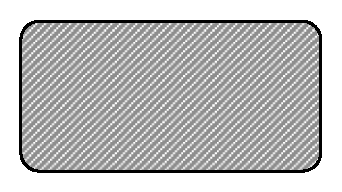
\epsfig{file=diagrams/kernel.eps,width=0.125\textwidth}} & %
\subfloat[Module-only instrumentation]{\hspace{2.5em}
\epsfig{file=diagrams/module.eps,width=0.125\textwidth}} \\
\subfloat[Module-only instrumentation, with a module function wrapped to run natively.]{\hspace{2.5em}
\epsfig{file=diagrams/module_wrapper.eps,width=0.125\textwidth}} & %
\subfloat[\label{fig:module_probe}Module-only instrumentation, with a kernel function wrapped to also be instrumented.]{\hspace{2.5em}
\epsfig{file=diagrams/module_probe.eps,width=0.125\textwidth}}
\end{tabularx}
\caption{\label{fig:granularities}Visual example of using different granularities of instrumentation to selectively instrument or not instrument specific code.}
\end{figure}

\subsection{Instrumenting Only Module Code}\label{sec:module}

Granary is the first kernel-space instrumentation system able to target instrumentation only at specific kernel modules, while executing the rest of the kernel natively and without overhead. Instrumenting only specific kernel modules is particularly useful for debugging tools because modules represent the bulk of new kernel code under development, and contain the most bugs \cite{FaultsInLinux}.

The basic technique that Granary uses to interpose on module code is hardware page protection. First, Granary page protects existing module code, marking it as non-executable. Then, Granary traps attempts to execute the protected module code and transparently recovers from these traps by returning execution to instrumented code. Granary also interposes on the Linux kernel's module loading process. When a kernel module is dynamically loaded, Granary bootstraps by page protecting the new module's code, and by translating the first basic block of the module's initialization function.  It then replaces the kernel's pointer to the native initialization function with a pointer to the translated basic block. The translation process continues when the kernel initializes the module by invoking the translated module code. 

While correct, hardware page protection is an inefficient mechanism for gaining control of module code execution. That is, after the (instrumented) module initializer runs to completion, Granary needs an efficient way to regain control of future invocations of the module's code. Our approach to regaining control is based on the observation that modules tell the kernel about their interfaces by registering interface functions with the kernel. These functions are the standard mechanism for extending the kernel's functionality. When the kernel executes a registered module function, control transfers from the kernel into the module. The act of registering a function is a signal to Granary that instrumentation must ``attach'' to the registered function when the kernel executes that function. In practice, when presented with such a signal, we would like to avoid the overhead of the trap that would occur when the registered function is executed by proactively replacing the registered function pointer with an instrumented equivalent.

Granary statically analyses of the kernel source code to discover potential attach points. Granary bridges the gap between static and dynamic analysis by using the static type information to generate code that dynamically discovers potential attach points. This code also gives tools type-safe access to the runtime object graph. The static analysis recognizes potential attach points as being: \begin{enumerate*}
	\item Function pointers passed as arguments to kernel functions.
	\item Function pointers stored in structures passed (by pointer or value) to kernel functions. This rule applies transitively. For example, if one structure has a field that points to another structure, and the latter structure contains a function pointer, then the latter structure's function pointers are also potential attach points. This is a common pattern in the Linux kernel, and mimics virtual tables in object-oriented languages.
	\item Function pointers and structures returned from attach points.
\end{enumerate*}

The code generation phase of Granary's static analysis creates ``wrappers'' for the kernel/module interface. Two kinds of wrappers are generated for the kernel/module interface: \begin{inparaenum}[i)]
	\item kernel function wrappers (\Cref{fig:function_wrapper}), and
	\item data-structure wrappers (called type wrappers).
\end{inparaenum} Kernel function wrappers are transparently invoked when module code attempts to invoke kernel code. Function wrappers delegate to type wrappers to find and wrap attach points passed to the kernel. 

%\begin{figure*}[t!]
%\lstset{language=C, tabsize=2, stepnumber=1}
%\begin{multicols}{2}
%\begin{lstlisting}[basicstyle=\scriptsize\ttfamily]
%struct device_driver {
%  ...
%  int  (*probe)(struct device *);
%  int  (*remove)(struct device *);
%  void (*shutdown)(struct device *);
%  int  (*suspend)(struct device *, pm_message_t);
%  int  (*resume)(struct device *);
%  ...
%  const struct dev_pm_ops *pm;
%  ...
%};
%\end{lstlisting}
%\columnbreak
%\begin{lstlisting}[basicstyle=\scriptsize\ttfamily]
%TYPE_WRAPPER(struct device_driver, {
%  PRE_OUT {
%    ABORT_IF_FUNCTION_IS_WRAPPED(arg.probe)
%    WRAP_FUNCTION(arg.probe);
%    WRAP_FUNCTION(arg.remove);
%    ...
%  }
%  POST_OUT {
%    POST_WRAP(arg.pm);
%  }
%})
%\end{lstlisting}
%\end{multicols}
%\caption{The Linux device driver structure is shown on the left. The automatically generated type wrapper for this structure is shown on the right. In the wrapper code, \texttt{arg} is a reference to a \texttt{struct device\_driver} object passed as, or referenced by, an argument to a kernel or module wrapper. Code in the \texttt{PRE\_OUT} section is applied to arguments of the wrapped type before a kernel wrapper is invoked. Similarly, code in the \texttt{POST\_OUT} section is applied to arguments of the wrapped type after a kernel wrapper is invoked. \texttt{POST\_WRAP} invokes the type wrapper that is specific to the value to which it is applied (\texttt{arg.pm}). Type wrappers also support \texttt{\_IN} suffixes instead of \texttt{\_OUT} suffixes, which apply to data going into modules (i.e., over module wrappers). Finally, the \texttt{RETURN\_} prefix is used to apply some code to return values of either kernel or module wrappers.}
%\label{fig:type_wrapper}
%\end{figure*}

\begin{figure}[t]
\lstset{language=C, tabsize=2, stepnumber=1}
\begin{lstlisting}[basicstyle=\scriptsize\ttfamily]
// struct inode *
// iget_locked(struct super_block *, unsigned long);
FUNCTION_WRAPPER(MODULE, iget_locked, (sb, ino), {
  PRE_OUT_WRAP(sb);
  struct inode *inode = iget_locked(sb, ino);
  POST_OUT_WRAP(sb);
  RETURN_IN_WRAP(inode);
  return inode;
})
\end{lstlisting}
\caption{\label{fig:function_wrapper}Atomatically generated wrapper for the \texttt{iget\_locked} kernel function. \texttt{iget\_locked} obtains an inode from a mounted file system. The super block argument (\texttt{sb}) is first pre-wrapped before it is passed to the original \texttt{iget\_locked} function. After \texttt{iget\_locked} returns, \texttt{sb} is then post-wrapped. Finally, the inode data structure returned by the kernel (\texttt{inode}) is return-wrapped and then returned to instrumented module code. The \texttt{OUT} and \texttt{IN} qualifiers of the wrappers denote the direction that data is travelling. \texttt{OUT}-wrappers apply to data passed from instrumented code out to the native code. \texttt{IN}-wrappers apply to data passed from native code into instrumented code.}
\end{figure}

If a pointer to a module function (a future attach point) is discovered, then Granary replaces that pointer with a function-specific \emph{module function wrapper}. Module function wrappers behave similarly to kernel function wrappers, in that they provide Granary more visibility into potential attach points, and provide instrumentation tools visibility into the runtime object graph.

\label{sec:wrappers}

Granary's wrappers expose a wealth of static program information to instrumentation tools. Instrumentation tools can use information present in wrappers to alter how code is instrumented, or to simply inspect the runtime object graph in a type-safe way. For example, we are actively using type information present in wrappers to create a tool that generates models of typical module behavior. The wrapper information serves two roles in our tool. First, we use type wrappers to assign type-specific IDs to module-allocated memory that is shared across the module/kernel interface. Type ID assignment is critical because it allows us to match memory reads and writes to specific kernel data structure fields. Second, we use the kernel and module function wrappers to generate call graphs of a module's execution. This call graph models module behavior (according to the kernel) because we label module code nodes with kernel data structure and function pointer field names (derived from module wrappers). This labelling allows us to generalize across similar modules. For example, code reached by calling the \texttt{ext4\_mount} and \texttt{btrfs\_mount} functions from the \texttt{ext4} and \texttt{btrfs} file system modules, respectively, are both labelled as \texttt{file\_system\_type::mount}, because the function addresses are stored (and later replaced by module wrappers) in the \texttt{mount} field of a \texttt{file\_system\_type} data structure. The combined records from multiple ``trusted'' modules of the same class (e.g., mature, open-source file systems) models the behavior of typical kernel modules. We hope that these models will help us build tools that classify and identify spurious module behavior. 

\subsection{Instrumenting Specific Functions}\label{sec:function_wrapper}

Instrumenting individual functions is useful when the code of interest is only a function or group of functions, or when the tool does not instrument all code, but wants visibility into functions that would otherwise execute natively. For example, \toolname{RCUdbg} interposes on the \texttt{rcu\_\linebreak[0]read\_\linebreak[0]lock} and \texttt{rcu\_\linebreak[0]read\_\linebreak[0]unlock} kernel functions. When \texttt{rcu\_\linebreak[0]read\_\linebreak[0]lock} is invoked by native kernel code, Granary attaches and begins instrumenting code using the read-side critical section instrumentation policy. When \texttt{rcu\_\linebreak[0]read\_\linebreak[0]lock} is invoked by instrumented code, Granary updates the nesting depth of the current read-side critical section. \texttt{rcu\_\linebreak[0]read\_\linebreak[0]unlock} behaves similarly.

Granary uses code splicing \cite{KernInst,AnyWhereAnyTimeDBT,KProbes} to allow tools to interpose on the execution of individual functions invoked by native code (which nornmally execute outside of Granary's control). Granary allows tools to interpose on specific functions invoked by instrumented code using kernel or module function wrappers (\Cref{sec:wrappers}). \Cref{fig:module_probe} is a visual example of how interposing on individual functions can be combined with module-only instrumentation to provide an instrumentation tool visibility into otherwise native kernel events.

\section{Runtime Instrumentation Code Specialization}\label{sec:how}

Existing instrumentation systems make it challenging to change how code is instrumented based on the runtime context. In practice, not all code needs or should be instrumented in the same way. Selectivity is on example of this: not all code needs to be instrumented, which is why Granary lets tools run some code natively and other code under instrumentation. Just as selectivity allows a tool to choose which code to instrument, specialization allows a tool to choose how to instrument that code. Specialization is especially useful for analysis tools that distinguish between light and heavyweight analyses, and for debugging tools that do different bug checks in different contexts.  For example, \toolname{RCUdbg} instruments code running inside RCU read-side critical sections differently from code running outside of read-side critical sections. Code is instrumented differently in these two contexts because a memory access that is valid inside of a read-side critical section can be invalid outside of a read-side critical section. If the instrumentation could not be specialized for these two different contexts, then \toolname{RCUdbg} would need insert instrumentation on every memory access that first determines the current context, and then performs the appropriate bug check. This additional check in the instrumentation introduces performance and space overheads (additional instructions) for \emph{all} memory instructions, as well as state management complexities for the runtime itself. That is, \toolname{RCUdbg} would need to track the current context in a reentrant way. %These additional overheads and complexities

%n doesn't just introduce performance and space (additional instructions) overheads on \emph{all} memory accesses, it also introduces complexity in terms of state management. That is, \toolname{RCUdbg} would need 

%Not all code needs to be or should be instrumented in the same way, just as not all code needs to be instrumented. 
%For code that is instrumented, having similar flexibility to selectivity is also useful: just
%just as instrumented code is a ``heavyweight" version of native code, so can 
%. In some cases, tools can distinguish between light and heavyweight instrumentation policies, just as instrumentation itself is a heavyweight version of native execution.
% However, not all code that is instrumented should have to be instrumented in the same way.
%For example, a security application could perform lightweight instrumentation of trusted kernel code, and more heavyweight instrumentation of untrusted modules.
%we want to change how code is instrumented when: \begin{enumerate}
%	\item {\bf Not all code needs to be instrumented in the same way.} This is an important concern when comprehensiveness isn't required, or when there are timing or performance constraints. For example, 
%	\item {\bf Different code should be instrumented differently.} For example, DBT-based sandboxing \cite{Vx32,ProgramShepherding} can be implemented by instrumenting trusted and untrusted code differently. In the case of the Linux, the kernel could be instrumented with a lightweight sandboxing policy for comprehensiveness, and untrusted modules could be instrumented with heavyweight policies for correctness.
%	\item {\bf The same code should be instrumented differently depending on the context.}
%\end{enumerate} 
%This is unfortunate, especially when the instrumentation is heavyweight, because then all instrumented code is slowed down equally. Some bugs are sensitive to 
%For analyses that must be run on production systems, 

%Granary gives tools the ability to be selective about what is instrumented. A natural extension of this selectivity is to allow tools to specialize how code is instrumented by dynamically switching the policy used to instrument code. Specialization is desirable in several cases. For example, some instrumentation is high-overhead, but does not need to be applied to all code. One example of this is Granary's \toolname{RCUdbg} tool, which instruments read-side critical sections more heavily than the rest of code. Unfortunately, existing DBT systems do not support runtime code specialization \cite{DRK,btkernel,Pin,DynamoRIO}. 

%To implement the equivalent of \toolname{RCUdbg}'s runtime code specialization using an existing DBT system requires that a tool developer maintain, update, and check runtime state to know whether or not code is executing inside or outside of a read-side critical section. If a basic block is executing in a read-side critical section, then instrumentation should be enabled, and if it's not in a read-side critical section then it should be disabled. Enabling/disabling instrumentation might be done at the instruction granularity, which introduces at least one branch instruction per native instruction, or at the granularity of basic blocks, which requires generating two copies of each native basic block, where a single branch at the beginning of a basic block chooses between the instrumented or uninstrumented version. Up until now, it has been assumed that there is a mechanism for maintaing state that consistently tracks the current execution context of kernel code (inside vs. outside of a read-side critical section). However, maintaining state in a way that is reentrant and resilient again arbitrary pre-emption and resumption is onerous.

Fortunately for tool developers, Granary has built-in support for runtime code specialization. Granary's implementation of runtime code specialization is unique in that: \begin{enumerate}

	\item {\bf It does not require manual state management.} Reentrant state management in the kernel environment is extremely complex. For example, using thread-private memory is a natural way to track the current execution context. However, there is no well-defined thread-private storage class in the Linux kernel. This is because interrupt handlers can, but don't always, share stacks with interrupted code, and interrupt handler code can swap out the current thread and swap in another thread. CPU-private storage is another option, but introduces an impedence mismatch on SMPs because contextual state is typically thread-specific, but a given thread can be rescheduled (e.g. by an interrupt) to execute on a different CPU. Finally, global state introduces potential performance bottlenecks (locking, false/true sharing) and sometimes tricky synchronization protocols.

	\item {\bf It does not require any runtime checking of the current runtime context.} If a tool like \toolname{RCUdbg} were implemented with DRK or btkernel, then \toolname{RCUdbg} would need to instrument code to continually check the current context and perform the correct memory access check given the current context. Checking the current context introduces performance overheads (additional instructions must be executed; branch mispredictions), and memory overheads (additional instructions are needed just to figure out what to check; icache misses).

\end{enumerate}

Granary's approach to runtime code specialization works by generating multiple versions of each basic block \emph{just-in-time}, where each version of a basic block is specialized to a different execution context.

% For example, in the Linux kernel, interrupt handling code can execute on the interrupted stack. If Granary is instrumenting all kernel code, the a tool developer needs to decide if the instrumented interrupt handling code should inherit the runtime context from the interrupted thread. Making such a judgement is further complicated by the fact that interrupt arrival and semantics are hardware-defined, but thread scheduling is software defined. That is, if an interrupt handler inherits 
%This results in less code cache bloat and more focused and simple instrumentation tools. That is, tool developers can focus on what the tool should do, rather than how to fit their idea of the tool
%	\item It works just-in-time, using basic block versioning, thus generating the minimum number of versio
% , and does not cause performance overheads by continually checking .
%Granary's approach to runtime code specialization 
 %uses a technique called \emph{context-driven instrumentation}.

\subsection{Specialization Using Basic Block Versions}\label{sec:policies}

%We developed a Granary tool that detects several Read-Copy-Update (RCU) API misuses in module code. Our tool focused on read-side critical sections (delimited by calls to \texttt{rcu\_read\_lock} and \texttt{rcu\_read\_unlock} in the code), however, most code executes outside of read-side critical sections. As an optimization, we wanted our heavyweight API-checking instrumentation to apply only when the code was executing within a read-side critical section. Implementing this optimization was challenging because each basic block was only translated once, and we had no way to know whether or not the heavyweight instrumentation should be applied to it. Knowing the state (within or outside a read-side critical section) at translation time was not sufficient, since the same translated block could later be executed in the opposite context. That is, code executing \emph{within} a read-side critical section may have originally been translated while executing \emph{outside} of a read-side critical section, and would thus omit the heavyweight API-checking instrumentation. This omission could cause our tool to miss bugs (i.e., it would not be comprehensive) when the basic block executes within a read-side critical section.

Granary tools can specialize instrumentation to the context in which the instrumented code will execute. Specialization is achieved by allowing multiple, differently instrumented versions of the same code to co-exist within Granary's code cache. That is, if the next basic block to execute has not yet been translated/instrumented for the current execution context, then a new version of that basic block will be created  specifically for the the current execution context.

%In the case of our \toolname{RCUdbg}, there were three execution contexts: within and outside of a read-side critical section. If the same module basic block is  executed in the two contexts, then Granary's code cache would contain two different instrumented versions of that basic block. The way that Granary distinguishes between different execution contexts is with \emph{instrumentation policies}. 

Granary tools identify execution contexts by creating instrumentation policies. An instrumentation policy is both a name for an execution context, as well as a function that decides how to instrument basic blocks that will execute within that context. All tools define an initial policy that Granary uses to instrument code. Tools are not limited to one policy though: any policy can declare a ``policy switch" that will take effect when a selected control-transferring instruction (CTI) is executed. Every policy function must declare what the ``next" policy to switch to will be. Policy switches can also be specified on a per-CTI basis. If a CTI has a specified policy, then any basic blocks targeted by that CTI will be instrumented by the specified policy. If a CTI does not have a specified policy, then it automatically inherits the next policy.

%The effect of a tool specifying a policy switch on a CTI is that the basic block(s) targeted by that CTI will be instrumented according to the specified policy. A CTI with an unspecified policy inherits its policy from its containing basic block. That is, if no policy is specified on a CTI, then

For example, \toolname{RCUdbg} defines three policies: $P_{read}$ for code executing within read-side critical sections, $P_{write}$ for code executing within write-side critical sections, and $P_{outside}$ for code executing outside of RCU read- and write-side critical sections. The following sequence of events describe some of the policy switching behavior of \toolname{RCUdbg} and how it interacts with block versioning.
\begin{enumerate*}
	\item Instrumentation begins with $P_{outside}$.
	\item $P_{outside}$ instruments a basic block containing a \texttt{call} to the \texttt{memset} kernel function. The \texttt{call} inherits the next policy, which is $P_{outside}$.
	\item When executed, the \texttt{call} to \texttt{memset} will cause \texttt{memset} to be instrumented by $P_{outside}$. No other instrumented versions of \texttt{memset} exist in Granary's code cache. Granary knows to use $P_{outside}$ and not another policy because $P_{outside}$ is stored in the edge data structure used by the first execution of the \texttt{call} (\Cref{sec:direct_control_flow}).
	\item Later, $P_{outside}$ instruments a basic block containing a \texttt{call} to \texttt{rcu\_\linebreak[0]read\_\linebreak[0]lock}. $P_{outside}$ sets next policy to $P_{read}$ and uses $P_{read}$ to instrument the tail of the basic block following the \texttt{call}.
	\item Execution naturally switches from being in one context (outside) into another (read) as execution returns from the \texttt{call} to \texttt{rcu\_\linebreak[0]read\_\linebreak[0]lock}. 
	\item $P_{read}$ instruments a basic block containing a \texttt{call} to \texttt{memset}. The \texttt{call} inherits the next policy, which is $P_{read}$.
	\item When executed, the \texttt{call} to \texttt{memset} within the read-side critical section will cause \texttt{memset} to be instrumented by $P_{read}$. There are now two versions of \texttt{memset} in the code cache: one specialized for executing outside of RCU-related code, and the other specialized to executing within read-side critical sections.
\end{enumerate*}

%For example, our \toolname{RCUdbg} invokes a policy switch from policy $P_{\mathit{null}}$ to policy $P_{\mathit{read\_critical}}$ when $P_{\mathit{null}}$'s instrumentation function observes a \texttt{call} instruction to the \texttt{rcu\_read\_lock} Linux kernel function. A similar switch occurs from $P_{\mathit{read\_critical}}$ back to $P_{\mathit{null}}$ at a \texttt{rcu\_read\_unlock}. Specialization that distinguishes between the inside and outside of read-side critical sections allows \toolname{RCUdbg} to do heavy-weight checks on functions like \texttt{memset}, but only when \texttt{memset} is invoked from within a read-side critical section.

The \toolname{RCUdbg} example highlights how the current execution context is implicity tracked by the current program counter or instruction pointer. Before the \texttt{call} to \texttt{rcu\_\linebreak[0]read\_\linebreak[0]lock}, the instructions were instrumented by $P_{outside}$. However, after the \texttt{call}, the instructions were instrumented by $P_{read}$. This insight reveals that policy switches and control-flow transfers behave like state transitions in a finite state machine, and that the program counter, by virtue of pointing at an instruction instrumented by a specific policy, tracks the current pogram state. This analogy, however, reveals a potential limitation: if RCU read-side critical sections are nested, then \toolname{RCUdbg}'s 3-state policy switching approach (as described) cannot distinguish a \texttt{call} to \texttt{rcu\_\linebreak[0]read\_\linebreak[0]unlock} from within an unnested and a nested read-side critical section. \toolname{RCUdbg} solves this problem by having more than one read policies: $P_{\mathit{{read}_0}}$, $P_{\mathit{{read}_1}}$, ..., $P_{\mathit{{read}_N}}$, which are generated on demand. In practice, this does not lead to code cache bloat because RCU read-side critical sections do not nest more than two times.

By default, Granary doesn't allow tools to specify policy switches on procedure return instructions (\texttt{ret}). This increases the ``power" of the formal model of policy switching from being a deterministic finite state automaton to being a restricted form of pushdown automaton. The program counter continues to track the current execution state, and saved program counters (returns addresses stored on the runtime call stack) record prior execution states. In this model, \texttt{call}s place contextual breadcrumbs (in the form of return addresses) on the runtime call stack, and \texttt{ret}s read these breadcrumbs to return to a previous context. For many tools, this is a natural model of state tracking as it is bound to the current thread, and because kernel code tends to follow a good call/return discipline.

%\toolname{RCUdbg} solves this problem by tracking the nesting depth using different read-policies ($P_{read}_0$, $P_{read}_1$, ...).

%Because policies name an execution context, they also represent states in a finite state machine. That is, code cache execution is in the state named by a policy if the  executing code was instrumented by that policy. A state transition occurs when control transfers from code instrumented by one policy to code instrumented by another policy. A limitation with this approach is that a single state does not encode the sequence of previous states that led to execution being in the current state. For example, RCU permits nested read-side critical sections. If two read-side critical sections are nested then switching from $P_{\mathit{read\_critical}}$ to $P_{\mathit{null}}$ on the first \texttt{call} to \texttt{rcu\_read\_unlock} meant that our tool would lose track of being in the context of the outer read-side critical section.  \toolname{RCUdbg} solves this problem by tracking the nesting depth of RCU read-side critical sections using policies, e.g. $P_{\mathit{read\_critical}_1}$, $P_{\mathit{read\_critical}_2}$, etc.

%An alternative and sometimes more powerful model for policy switching is to prevent policy switching on function return instructions (e.g. either through manually specifying a policy switch, or by inheriting the policy from the basic block containing the \texttt{ret} instruction). In most cases, function returns are natural policy reverting points. This is because the current instruction pointer (program counter) encodes the current execution context (by being in a basic block instrumented by some policy), and the code cache return addresses stored on the runtime call stack encode all previous execution contexts. This asymmetry between \texttt{call}s and \texttt{ret}s yields a more powerful context-tracking state machine: \texttt{call}s place contextual breadcrumbs (in the form of return addresses) on the runtime call stack, and \texttt{ret}s read these breadcrumbs to return to a previous context. Policy switches under this lens behave similarly to state transitions in a pushdown automaton; \texttt{call} instructions push a new state onto the stack for each function, \texttt{ret} instructions pop the current function's state from the stack, and other CTIs induce state transitions within the current function by altering control flow.

Granary implements policy tracking and switching by encoding policy information into the meta-data of basic blocks, the instructions of in-edge code generated for indirect control flow, and the edge data structures used by direct control flow. When an instrumented CTI executes for the first time, it yields control to Granary with the CTI target and policy information as inputs. Granary decodes and instruments the targeted instructions according to the input policy information.

% CTIs of basic blocks. \Cref{fig:direct_edge_code} shows an example of how policy information is directly recorded into control-transfer edge code. If a policy switch is not specified on an instrumented CTI then that CTI inherits the policy used to instrument the basic block containing the CTI. 

\subsection{Partial Specialization Using Policy Properties}

Granary internally specializes code at a finer granularity than that described by a tool's instrumentation policies. Granary will sometimes generate multiple versions of a given basic block, even for the same instrumentation policy. Other times, Granary will only generate extra entries in the code cache index that are eventually disambiguated. When apparently redundant code generation occurs, it means that certain properties that are internally tracked by Granary are present, and that these properties affect how Granary or its tools can optimize or instrument code. 

For example, Granary tracks whether code may or may not access user space data, because this code can potentially result in a page fault. Granary can detect this code using a combination of pattern recognition, and policy property propagation. This internal mechanism is needed to correctly handle page faults in instrumented kernel code (\Cref{sec:interrupt_return_address_transparency}), and is also useful for optimizing code generated by tools as well. For example, Granary's \toolname{BoundsChecker} tool alters the 16 high order bits of addresses returned from kernel allocators, to make it easy to associate bounds information with each allocated object \cite{BehaveOrBeWatched}. Checked and unchecked kernel addresses can distinguished by testing only a single bit. However, user space addresses and checked addresses are harder to distinguish, requiring two bits to be checked.  Fortunately,  few instructions dereference user space addresses, and Granary tracks whichs basic blocks might contain those instructions, thus allowing the \toolname{BoundsChecker} to avoid many unnecessary bit tests.

Another example of partial specialization that benefits instrumentation tools is Granary's SIMD register tracking property. Granary detects and tracks the usage of SIMD registers (\texttt{\%xmm0} through \texttt{\%xmm16}). This informs instrumentation tools on when its safe to save transient data to the SIMD registers instead of to memory, which can result in improved performance \cite{Minemu}.

%An access to user space data can potentially cause a fault in the kernel . Code that accesses user space data contains specify binary patterns; however, sometimes those patterns are not present in the individual basic blocks that dereference the user space address. 

%For example, Granary's address watchpoints framework uses address tainting to easily associate meta-data to allocated objects, and to make it easy to distinguish between tracked and untracked objects \cite{BehaveOrBeWatched}. The mechanism used to taint an address depends on x86-64 ``non-canonical" addresses. A canonical address has all of its 16 high-order bits set to 0 or set to 1. In Linux, the 16 high-order bits of kernel addresses are all 1, and the 16 high-order

%These propeties, called policy properties, transparently persist across control-flow instructions, even if the CTI changes the current policy. Granary tracks the following policy properties:

%\begin{description}
%	\item[Temporary]
%	\item {\bf Kernel vs. module code.}
%	\item 
%	\item {\bf SIMD register usage.}
%\end{description}


\section{Application: Control-Flow Graphs}\label{sec:cfg}

\section{Application: RCUdbg}\label{sec:rcudbg}

Read-Copy-Update (RCU) is a scalable, lock-free synchronization mechanism used in the Linux kernel \cite{RCU,RCUInLinux}. When correctly used, RCU permits concurrent reads and writes to shared data structures, but requires that writers synchronize among themselves. Like other synchronization mechanisms, RCU has a deceptively simple API. Misuses of the API can result in hard-to-find bugs that can be implementation-specific (i.e. bugs that manifest in one version of RCU but not another) or architecture-specific (e.g. bugs that only exhibit on architectures with a relaxed memory model). For example, RCU bugs sometimes manifest as use-after-free bugs, which can result in silent data corruption (if the underlying memory remains used) or kernel panics. 

% (assuming that pointer reachability is sufficient to determine semantic reachability in this case).

Granary's \toolname{RCUdbg} tool is designed to catch RCU bugs related to kernel code misusing pointers to RCU-protected data structures. The following is a non-exhaustive list of requirements that must be met by reader and writer threads operating on an RCU-protected data structure. The list omits a description of how RCU-protected data structures are garbage collected, which is beyond the scope of the bugs caught by \toolname{RCUdbg}.

%the associated memory may or may not be free, but the data structure occupying that memory can't be proven to exist. This 
%  However, this class of RCU bugs is not well-suited to being detected by a use-after-free memory checker tool
%RCU is notoriously hard to use, despite its relatively simple API. RCU usage bugs, like bugs with other synchronization mechanisms, often stay hidden and only exhibit themselves for very specific thread interleavings/schedules.
% go silently unnoticed because the memory 
%While bugs related to mutual exlusion locks might result in easily observable deadlocks, bugs related to RCU typically result in use-after-free errors, which sometimes go silently unnoticed, sometimes result in kernel panics, and most of the time work as expected because the associated data is .

\begin{enumerate}
	\item Readers must tolerate an inconsistent view of the shared data structure. That is, a reader operating concurrently with a writer might observe either the version of the data before or after the writer's changes have been published. This can be complicated when writers perform multiple, discrete updates to a data structure. One example of this is a doubly linked list: a writer that is adding a new entry into a doubly linked list must update at least two RCU-protected pointers.
	
	\item Readers must operate within \emph{read-side} critical sections, which are delimited by \texttt{rcu\_read\_lock} and \texttt{rcu\_read\_unlock}, respectively.
	
	\item Within read-side critical sections, readers can only read a shared data structure after obtaining a pointer to that shared data structure using the \texttt{rcu\_dereference} API function. An RCU-protected pointer is like a normal pointer, but points to a potentially incomplete or partially-constructed data structure. \texttt{rcu\_dereference} operates on an RCU-protected pointer and returns an ``unprotected" version of the pointer. The reader can use the unprotected pointer to safely access the shared data structure within the remainder of the its read-side critical section. If \texttt{rcu\_dereference} is not used, then the reader might observe a partially-constructed (i.e. incomplete) version of the shared data structure. Notably, accessing the original data structure and not the dereferenced data structure pointer--even after an \texttt{rcu\_dereference}--is undefined behavior. That is, within a read-side critical section, RCU only guarantees the ``completeness" of data structures pointed to by RCU-dereferenced pointers. Data accessed within a read-side critical section is \emph{not} guaranteed to exist outside the read-side critical section.

	\item Writers must synchronize among themselves before any writes to a shared data structure are performed. Synchronization is typically achieved via mutual exclusion locks, spin locks, or by having a single, designated writer thread. We say writes to the shared data structure occur within \emph{write-side} critical sections.

	\item RCU only defines how writers can update RCU-protected pointer within a shared data structure. Modification of non-RCU-protected pointer fields within an RCU-protected data structure is beyond the scope of RCU's correctness guarantees.

	\item Writers wishing to update an RCU-protected pointer in a shared data structure must use the \texttt{rcu\_assign\_pointer} API function. \texttt{rcu\_assign\_pointer} assigns a new value to an RCU-protected pointer in a shared data structure.

	\item Readers must access any pointer field operated on by an \texttt{rcu\_\linebreak[0]assign\_pointer} using \texttt{rcu\_\linebreak[0]dereference}. For example, if the \texttt{next} pointer field in \emph{any} list element of an RCU-protected list has been assigned to by \texttt{rcu\_assign\_\linebreak[0]pointer}, then \emph{all} \texttt{next} pointer fields must be accessed by readers of that list by using \texttt{rcu\_\linebreak[0]dereference}. In this sense, using \texttt{rcu\_\linebreak[0]dereference} and \texttt{rcu\_assign\_\linebreak[0]pointer} marks specific variables and data type fields as containing RCU-protected pointers.

\end{enumerate}

% NOTE!!!!
%
% All of those spaces before /* BUG! */ and such are so that the lstlisting will be *close* to the columnwidth!! Somehow linewidth param of lstset didn't work for me :-(

\lstset{
	language=C,
	tabsize=2,
	stepnumber=1,
	morekeywords={rcu_read_lock,rcu_dereference,rcu_read_unlock,rcu_assign_pointer,spin_lock,spin_unlock}}

% Example code showing an existence bug.
\newsavebox\rcuexistencebug
\begin{lrbox}{\rcuexistencebug}
\begin{lstlisting}[basicstyle=\scriptsize\ttfamily]
rcu_read_lock();
  elm = rcu_dereference(list_head);
  data = elm->data;                  /* Valid */
rcu_read_unlock();
data = elm->data;                     /* BUG! */
\end{lstlisting}
\end{lrbox}

% Example code showing another existence bug.
\newsavebox\rcuderefbug
\begin{lrbox}{\rcuderefbug}
\begin{lstlisting}[basicstyle=\scriptsize\ttfamily]
rcu_read_lock();
  elm = rcu_dereference(list_head);
  if(elm != NULL)
    data = list_head->data;           /* BUG! */
rcu_read_unlock();
\end{lstlisting}
\end{lrbox}

% Example code showing another existence bug.
\newsavebox\rcuassignderefbug
\begin{lrbox}{\rcuassignderefbug}
\begin{lstlisting}[basicstyle=\scriptsize\ttfamily]
spin_lock();
  elm = kmalloc(...);
  elm->next = list_head->next;
  rcu_assign_pointer(list_head->next, elm);
spin_unlock();
...
rcu_read_lock();
  elm = rcu_dereference(list_head);
  while(elm != NULL) {
    data += elm->data;
    elm = elm->next;                  /* BUG! */
  }
rcu_read_unlock();
\end{lstlisting}
\end{lrbox}

\begin{figure}[ht!] %
\subfloat[\label{fig:rcu_existence_bug}Despite correctly obtaining a pointer to a shared data structure using \texttt{rcu\_dereference} within a read-side critical section, properties (2) and (3) tell us that the data pointed to by \texttt{elm} is not guaranteed to exist after the read-side critical section ends.]{\fbox{\usebox\rcuexistencebug}} %

\subfloat[\label{fig:rcu_deref_bug}Despite the call to \texttt{rcu\_dereference}, properties (1) and (3) tell us that \texttt{list\_head} is not guaranteed to be equivalent to \texttt{elm} because a writer might have concurrently changed the value of the \texttt{list\_head} pointer. That is, if \texttt{elm} is non-\texttt{NULL}, then the data pointed to by \texttt{elm} is guaranteed to exist for the remainder of the read-side critical section. However, the value of \texttt{list\_head} is \emph{not} guaranteed to remain consistent--even within read-side critical sections--and so \texttt{list\_head} might point to a \texttt{NULL} pointer when \texttt{elm} does not.]{\fbox{\usebox\rcuderefbug}} %

\subfloat[\label{fig:rcu_assign_bug}This example shows the code for a writer thread adding a new element into the second position of an RCU-protected list. The code for reader threads is also shown, where readers iterate over the list by traversing \texttt{next} pointers and sum up the \texttt{data} fields of each visited list element. The access of \texttt{elm->next} violates of properties (3) and (7). That is, the next element of the list is only guaranteed to be fully constructed within the read-side critical section if the reader executes \texttt{rcu\_dereference(elm->next)}. Therefore, the first read of \texttt{elm->next} might yield a pointer to partially constructed data.  Because that data is not guaranteed to be fully constructed, the next read of \texttt{elm->next} (i.e. \texttt{elm->next->next}) might read an invalid pointer from uninitialized memory. Treating the value of uninitialized memory as a valid pointer could trigger a kernel panic or silent data corruption.]{\fbox{\usebox\rcuassignderefbug}} %
\caption{\label{fig:rcu_bugs}Example RCU bugs related to misuses of RCU-protected pointers.}
\end{figure}

\toolname{RCUdbg} is primarily concerned with finding bugs related to RCU-rpotected pointer misuses by reader threads (both inside and outside of read-side critical sections). As mentioned above, RCU bugs sometimes manifest as use-after-free bugs. Unfortunately, a pure use-after-free-based checking approach is insufficient (\Cref{fig:rcu_assign_bug} is one such example). \Cref{fig:rcu_existence_bug} is an example of an RCU usage bug that can manifest as a use-after-free bug if one is unlucky enough to observe a very specific thread schedule. Suppose that execution is interrupted after \texttt{rcu\_read\_unlock}, but before the access to \texttt{elm->data}. If \texttt{elm} is garbage collected and freed before the code resumes its execution, then the access to \texttt{elm->data} is a use-after-free bug. This kind of bug is a time bomb waiting to go off. Fortunately, \toolname{RCUdbg} catches the bug in \Cref{fig:rcu_existence_bug} right when \texttt{elm->data} is accessed.


%\Cref{fig:rcu_bugs} shows some example usages of RCU, and some of the more subtle pointer-related bugs that can happen because of the interaction of rules (1), (2), (3), and (7).


\toolname{RCUdbg} detects the the following RCU bugs related to misuses of RCU-protected pointers.
\begin{itemize}[leftmargin=3.2em]
	\item[B1)] Reads through an RCU-dereferenced pointer outside of a read-side critical section (\Cref{fig:rcu_existence_bug}).
	\item[B2)] Reads through an RCU-dereferenced pointer in the wrong read-side critical section.

	\item[B2)] Reads through an RCU-assigned pointer that don't first use \texttt{rcu\_dereference} (\Cref{fig:rcu_deref_bug}).
	\item[B3)] Reads through fields of RCU-protected data structures that should be accessed via \texttt{rcu\_dereference} (\Cref{fig:rcu_assign_bug}).
	
	\item[B5)] Writes through an RCU-dereferenced pointer.
	\item[B6)] Writes through an RCU-assigned pointer by a non-write thread.
\end{itemize}

Bugs B1 and B2 relate to whether or not we can prove that a given RCU protected data structure exists. Bugs B2 and B3 relate to whether or not a given RCU protected data structure has been fully constructed. Finally, bugs B5 and B6 relate to invalid uses RCU-protected and RCU-unprotected pointers, where correct synchronization among writers is not maintained.

% or is constructed at a given program point. Bugs B2 through B

% of this class of RCU bugs is proof-of-existence or proof-of-constructedness bugs. That is, an RCU-protected data structue exists if it is \emph{reachable} (i.e. by at least one reader thread), and if it is \emph{fully constructed} (i.e. all fields or components of the data structure have been initialized). 

\toolname{RCUdbg} gains visibility on RCU operations in two ways: \begin{enumerate}
	\item The Linux kernel RCU implementation is annotated to provide more information to \toolname{RCUdbg}. This information includes source code file and line information for bug reporting, and additional memory references that \toolname{RCUdbg} uses to get better visibility on bugs. These annotations are strictly internal to the RCU API, and thus require no changes to code using this API.
	\item The annotated RCU API functions are specialized using Granary's function wrapping feature (\Cref{sec:function_wrapper}). Specifically, 
\end{enumerate}

%\toolname{RCUdbg} interposes on an annotations are added into the Linux kernel's RCU implementation. These annotations 


%uses Granary's address watchpoints feature \cite{BehaveOrBeWatched} to ``taint" addresses participating in RCU-protected data structures. 

%Function wrappers are used to specialize the execution of \texttt{rcu\_\linebreak[0]dereference} and \texttt{rcu\_assign\_\linebreak[0]pointer}:

\begin{figure}[t!]
\lstset{language=C, tabsize=2, stepnumber=1}
\begin{lstlisting}[basicstyle=\scriptsize\ttfamily]
// As used in the code:
//   p = rcu_dereference(q);
// Internally annotated to become:
//   p = __rcudbg_deref(&q, q);
// Wrapper:
FUNCTION_WRAPPER(__rcudbg_deref, (q_addr, q), {
  if(is_watched_address(q_addr)) {
    // Make sure q_addr
  } else {

  }
  return add_watchoint(q, DEREF);
})
\end{lstlisting}
\caption{}
\label{fig:rcu_dereference_wrapper}
\end{figure}

%\begin{center}
%\begin{minipage}{0.6\columnwidth}
%\begin{lstlisting}[basicstyle=\scriptsize\ttfamily]
%elm = rcu_dereference(list_head);
%\end{lstlisting}
%\end{minipage}
%\end{center}
%
%Becomes:
%
%\begin{center}
%\begin{minipage}{0.8\columnwidth}
%\begin{lstlisting}[basicstyle=\scriptsize\ttfamily]
%elm = deref_taint(rcu_dereference(list_head));
%\end{lstlisting}
%\end{minipage}
%\end{center}
%
%Tainted addresses are introduced in two ways:
%\begin{description}
%	\item[\texttt{rcu\_assign\_pointer}] operates on two pointers: 
%	\item[\texttt{rcu\_dereference}] operates on a potentially tainted pointer (as introduced by \texttt{rcu\_assign\_\linebreak[0]pointer}, and returns a deref-tainted pointer.
%\end{description}
%

%Unfortunately, approaching RCU bug detection from the perspective of finding use-after-free errors is insufficient. Use-after-free detection attacks a symptom of the problem that is highly dependent on thread interleavings and scheduling. That is, RCU can be misused in a way that results in very unlikely, but potential use-after-free bugs. An example of this case is when a writer thread, operating on a RCU-protected linked list, unlinks an element and queues its memory for later freeing. RCU provides a mechanism whereby readers can safely access this element for a brief period of time (called a read-side critical section). When the memory is eventually freed depends is implementation-defined, but depends on other reader activity.

%How soon after a read-side critical section ends 

% There are many cases readers can access an RCU-protected data structure because they have not been freed \emph{yet}


%

% a data structure cannot be proven to exist at some potentially allocated memory. Existence in this case relates to semantic reachability. For example, if a list element $E_n$ from an RCU-protected list is reachable from the head of the list by traversing zero-or-more intermediate elements $E_0, ..., E_{n-1}$, then $E_n$ is said to exist. While related, memory leak detection (e.g. via conservate mark and sweep) is also insufficient for ladidadidaaaa TODO TODO TODO

\section{Evaluation}\label{sec:eval}

What has been evaluated:

\paragraph{lmbench}
\begin{itemize}
	\item Btkernel
	\item Granary, full-kernel, null
	\item Granary, full-kernel, even/odd
	\item Granary, full-kernel, even/odd, where even/odd is a runtime check and branch.
\end{itemize}

\paragraph{fileserver}
Setup: 1GB RAM, 3GB partition, ext3+jbd, >1GB mounted file system.
\begin{itemize}
	\item full-kernel
	\begin{itemize}
		\item Btkernel
		\item Granary, null
		\item Granary, even/odd
		\item Granary, even/odd, where even/odd is a runtime check and branch.
	\end{itemize}
	\item module-only, (ext3+jbd)
	\begin{itemize}
		\item Granary, null
		\item Granary, even/odd
		\item Granary, even/odd, where even/odd is a runtime check and branch.
	\end{itemize}
\end{itemize}

\paragraph{kernel compile}
Same as fileserver, but with 8GB RAM instead of 3GB.

\paragraph{recursive copy of kernel source tree}
Same as fileserver, but with 8GB RAM instead of 3GB.

\section{Related Work}\label{sec:related}
Prior work can be classified as either whole-kernel/system DBT, or probe-based kernel instrumentation. We discuss how Granary differs from these approaches.
\paragraph{Whole-kernel/system DBT}
PinOS \cite{PinOS} is a port of the Pin \cite{Pin} DBT framework that performs whole-system instrumentation. It has high overheads and depends on hardware virtualization, which prevents it from instrumenting non-virtualizable kernel modules. 

QMEU is a flexible, whole-system emulator with kernel-level paravirtualization support (using KVM) \cite{QEMU}. Like PinOS, QEMU cannot instrument non-virtualizable device drivers.

DRK \cite{DRK} is a kernel space port of the DynamoRIO \cite{DynamoRIO} DBT framework. DRK instruments the entire kernel and all device drivers/modules. DRK follows a strict transparency model, which limits the flexibility of instrumentation and increases overheads. 

Btkernel is a fast and scalable system for the kernel \cite{btkernel}. Like Granary, but unlike DRK, btkernel applies a relaxed transparency model when instrumenting the kernel. For exmaple, code cache addresses are exposed to the instrumented kernel in the form of function call return addresses and interrupt return addresses. Unlike Granary, btkernel operates using an instruction translation ``rulebook", which limits instrumentation to being defined ahead-of-time, on a per-instruction basis. Btkernel does not support any form of runtime code specialization. That is, like DRK, btkernel instruments all code, but cannot change the granularity of instrumentation or the instrumentation policy applied to code.

TODO: JIFL

\paragraph{Probe-based Instrumentation} Several systems support injecting code at specific locations within kernel code.

TODO: SystemTap

KernInst \cite{KernInst} can inject code at almost any location in an unmodified commodity OS. By default, KernInst uses debugging information normally present in kernel binaries to specify probe-points; however, absolute memory addresses can also be provided.

Other examples with similar or more restricted functionality include LTTng \cite{LTTng}, KProbes \cite{KProbes}, DProbes \cite{DProbes}, and ftrace \cite{ftrace}. These systems are unable to perform fine-grained instrumentation of instructions or memory.


\section{Conclusion}\label{sec:conclusion}
%We created Granary to address the challenges of instrumenting binary kernel modules.  Granary provides mixed-mode execution to remove the overheads of DBT for uninstrumented kernel code.  A relaxed transparency model further improves performance and allows greater visibility into the interactions between module and kernel code.  Granary also supports policy-driven instrumentation, which allows tools to specialize their instrumentation based on the context in which code executes.  Finally, Granary exposes high-level static analysis information to dynamic instrumentation tools, making it easy to match low-level memory reads with specific fields in data structures at the source code level. 

%Together, Granary's features simplify the development of powerful kernel module analysis tools, while delivering lower overheads than previous kernel dynamic binary instrumentation solutions.



\bibliographystyle{acm}
\bibliography{library}

\end{document}
